% ============================================================
% MIDWAY 1 PRESENTATION  (revision 3)
% Learning Topological Phases from Quantum Geometry
% Structure: title + 6 main slides + appendix (derivations, numerics)
% Compile twice (pdflatex). Needs: appendixnumberbeamer (texlive-latex-extra).
% ============================================================

\documentclass[aspectratio=169,11pt]{beamer}

\usepackage[T1]{fontenc}
\usepackage{lmodern}
\usepackage{amsmath}
\usepackage{amssymb}
\usepackage{bm}
\usepackage{graphicx}
\usepackage{booktabs}
\usepackage{array}
\usepackage{appendixnumberbeamer}

\usetheme{Madrid}
\setbeamertemplate{navigation symbols}{}
\setbeamerfont{frametitle}{size=\normalsize}

\setbeamertemplate{footline}{
    \leavevmode
    \hbox{
        \begin{beamercolorbox}[wd=.80\paperwidth,ht=2.5ex,dp=1ex,leftskip=1em]{author in head/foot}
            \insertshortauthor\hspace{1em}\insertshorttitle
        \end{beamercolorbox}
        \begin{beamercolorbox}[wd=.20\paperwidth,ht=2.5ex,dp=1ex,center]{date in head/foot}
            \insertframenumber/\inserttotalframenumber
        \end{beamercolorbox}
    }
}

% ---------- compact spacing ----------
\setlength{\parskip}{0pt}
\setlength{\columnsep}{0.45cm}
\setlength{\abovedisplayskip}{2pt plus 1pt minus 1pt}
\setlength{\belowdisplayskip}{2pt plus 1pt minus 1pt}
\setlength{\abovedisplayshortskip}{1pt plus 1pt minus 1pt}
\setlength{\belowdisplayshortskip}{1pt plus 1pt minus 1pt}
\setlength{\leftmargini}{1.3em}
\setlength{\tabcolsep}{4pt}

% ---------- notation ----------
\newcommand{\ML}{\mathrm{ML}}
\newcommand{\NUM}{\mathrm{num}}
\newcommand{\ANA}{\mathrm{ana}}

% ---------- boxes ----------
\setbeamercolor{ResearchBox}{bg=blue!5,fg=black}
\setbeamercolor{ResultBox}{bg=green!5,fg=black}
\setbeamercolor{WarnBox}{bg=red!8,fg=black}

\newenvironment{ResearchBox}
{\begin{beamercolorbox}[rounded=true,sep=0.45em]{ResearchBox}}
{\end{beamercolorbox}}
\newenvironment{ResultBox}
{\begin{beamercolorbox}[rounded=true,sep=0.40em]{ResultBox}}
{\end{beamercolorbox}}
\newenvironment{WarnBox}
{\begin{beamercolorbox}[rounded=true,sep=0.40em]{WarnBox}}
{\end{beamercolorbox}}

% ---------- title info ----------
\title[Learning Topological Phases]{Learning Topological Phases from Quantum Geometry}
\subtitle{Machine Learning of Quantum Geometric Tensor Fields}
\author[Rajat Shuvra Saha]{Rajat Shuvra Saha}
\institute[NISER]{National Institute of Science Education and Research\\Bhubaneswar}
\date{05 October 2026}

\begin{document}

% ============================================================
% TITLE
% ============================================================
\begin{frame}[plain]
\centering
\vspace{0.55cm}
{\LARGE\bfseries Learning Topological Phases\\from Quantum Geometry}

\vspace{0.30cm}
{\large Machine Learning of Quantum Geometric Tensor Fields}

\vspace{0.75cm}
{\large\bfseries Rajat Shuvra Saha}

\vspace{0.15cm}
National Institute of Science Education and Research\\Bhubaneswar

\vfill
{\large\bfseries Progress Update-1}

\vspace{0.12cm}
05th--06th October 2026
\end{frame}


% ============================================================
% 1. BASE PAPER
% ============================================================
\begin{frame}{1. Base paper and how it inspired us}
\footnotesize

\begin{ResearchBox}\scriptsize
\textbf{Base paper:} A.-K.~Wu, L.~Primeau, J.~Zhang, K.~Sun, Y.~Zhang, S.-Z.~Lin,
``Modeling quantum geometry for fractional Chern insulators with unsupervised learning,''
\textit{npj Comput.\ Mater.} \textbf{12}, 280 (2026), doi:10.1038/s41524-026-02155-1
\end{ResearchBox}

\vspace{0.10cm}

\begin{columns}[T]
\begin{column}{0.49\textwidth}
\textbf{What the paper does}
\begin{itemize}
    \item Learns form factors
    $\lambda_{\mathbf q}(\mathbf k)=\langle u_{\mathbf k}|u_{\mathbf k+\mathbf q}\rangle$
    with a VAE and PCA.
    \item Data \textbf{generated from a physical Hamiltonian} (QBCP); no database.
    \item Latent space separates FCI from non-FCI \emph{without labels}.
    \item PCA modes carry approximately quantized Chern numbers:
    \textbf{global topology is encoded in local geometry}.
    \item Gauge-invariant $\Omega$, $g$ via Wilson loops.
\end{itemize}
\end{column}

\begin{column}{0.49\textwidth}
\textbf{How it inspired our project}
\begin{enumerate}
    \item \textbf{Self-generated data} from analytic two-band Hamiltonians.
    \item \textbf{BZ fields as images:} periodic-padded convolutions.
    \item \textbf{Local $\rightarrow$ global:} our research question.
    \item \textbf{Outlook (conv.\ + attention):} attention-pooling global branch.
    \item \textbf{Gauge-free inputs:} built from $\mathbf d(\mathbf k)$.
\end{enumerate}
\end{column}
\end{columns}

\vspace{0.10cm}
\begin{ResultBox}\centering\scriptsize
\textbf{Where we differ:} supervised and physics-informed (not unsupervised);
single-particle Chern/$\mathbb Z_2$ topology (not many-body FCI);
outputs are local QGT fields plus a topological class.
\end{ResultBox}
\end{frame}


% ============================================================
% 2. PROBLEM SETUP AND DATA
% ============================================================
\begin{frame}{2. Problem setup and data}
\footnotesize

\begin{columns}[T]
\begin{column}{0.50\textwidth}
\textbf{Research question:} can a network infer global topology from local
quantum-geometric fields?

\vspace{0.08cm}
\textbf{Quantum geometric tensor} ($P$ = occupied-band projector)
\[
Q_{ij}=\operatorname{Tr}[P\,\partial_iP\,\partial_jP]=g_{ij}-\tfrac{i}{2}\Omega_{ij}
\]

\textbf{Input} $X_{\rm loc}\in\mathbb R^{19\times40\times40}$:\\
{\scriptsize $\mathbf d,\hat{\mathbf d},\partial_x\hat{\mathbf d},\partial_y\hat{\mathbf d},
\nabla^2\hat{\mathbf d},|\mathbf d|,|\mathbf d|^{-1},|\partial_x\hat{\mathbf d}|,|\partial_y\hat{\mathbf d}|$}

\textbf{Output:} $g^{\ML}_{xx},g^{\ML}_{xy},g^{\ML}_{yy},\Omega^{\ML}_{xy}$ (shape $4\times40\times40$)
and $C^{\ML}\in\{-1,0,+1\}$.

\vspace{0.08cm}
\begin{ResearchBox}\scriptsize
Indexing Used: \\
$\ML$ = network prediction;\\ $\NUM$ = computed from $H(\mathbf k)$;\\
$\ANA$ = closed form.
\end{ResearchBox}
\end{column}

\begin{column}{0.47\textwidth}
\textbf{What does our Data look like?}
\begin{itemize}
    \item \textbf{Synthetic, generated by our script}
    No QWZ dataset borrowed; no external database
    (JARVIS is the later stage).
    \item Family: randomized generalized two-band
    $H=\mathbf d(\mathbf k)\!\cdot\!\boldsymbol\sigma$; contains QWZ as a special case.
    \item Exact analytic $g_{ij}$, $\Omega_{xy}$ and $C$ labels.
    \item Tensors: $X$: $(225,19,40,40)$, $Y$: $(225,4,40,40)$.
    \item Balanced: 75 samples each for $C=-1,0,+1$.
    \item Gap: min $=0.403$, mean $=1.009$ (cut $\geq0.4$).
\end{itemize}
\end{column}
\end{columns}
\end{frame}


% ============================================================
% 3. MODEL AND TRAINING
% ============================================================
\begin{frame}{3. Model, loss and training}
\footnotesize

\begin{columns}[T]
\begin{column}{0.46\textwidth}
\textbf{\texttt{PhysicsQGTNet}}
\begin{itemize}
    \item Local branch + multi-scale periodic U-Net (3-level decoder).
    \item Attention-pooling global branch $\rightarrow$ Chern classifier.
    \item Circular padding on the BZ torus.
\end{itemize}

\textbf{Physics-informed loss}
{\scriptsize
\[
\mathcal L=4\mathcal L_{\rm QGT}+\mathcal L_{\rm geo}+2\mathcal L_{\rm topo}+\tfrac12\mathcal L_{\rm cls}
\]}
\vspace{-3mm}

{\scriptsize $\mathcal L_{\rm geo}$ enforces $\det g=\Omega_{xy}^2/4$;\\\\
$\mathcal L_{\rm topo}$ uses $C^{\ML}=\frac1{2\pi}\!\int\!\Omega^{\ML}_{xy}d^2k$.}
\end{column}

\begin{column}{0.51\textwidth}
\centering
\textbf{Training log, 100 epochs (train metrics)}

\vspace{0.05cm}
\scriptsize
\renewcommand{\arraystretch}{1.08}
\begin{tabular}{@{}lrrr@{}}
\toprule
 & Ep.\ 1 & Ep.\ 40 & Ep.\ 100\\
\midrule
Total loss & 6.036 & 0.00951 & 0.00193\\
$\mathcal L_{\rm QGT}$ & 0.0291 & 0.00161 & 0.00030\\
$\mathcal L_{\rm geo}$ & 0.0418 & 0.00311 & 0.00107\\
$\mathcal L_{\rm topo}$ & 0.4343 & 0.00019 & 0.00004\\
C-cls acc. & 0.449 & 1.000 & 1.000\\
C-int MAE & 0.555 & 0.0075 & 0.0030\\
\bottomrule
\end{tabular}
\end{column}
\end{columns}

\vspace{0.10cm}
\end{frame}


% ============================================================
% 4. QWZ BENCHMARK
% ============================================================
\begin{frame}{4. QWZ benchmark: analytical reference vs.\ ML}
\footnotesize

\begin{columns}[T]
\begin{column}{0.40\textwidth}
\textbf{Exact QWZ scan}, boundaries $m=-2,0,+2$

\vspace{0.06cm}
\renewcommand{\arraystretch}{1.1}
\begin{tabular}{@{}lr@{}}
\toprule
Metric & Value\\
\midrule
Classifier accuracy & 0.466\\
Classifier macro-F1 & 0.274\\
Integrated-$C$ MAE & 0.733\\
Integrated-$C$ RMSE & 0.935\\
Mean field RMSE & 0.299\\
\midrule
Val.\ QGT MSE & 0.0401\\
Val.\ round-$C$ acc. & 0.667\\
\bottomrule
\end{tabular}

\vspace{0.12cm}
\begin{ResultBox}\scriptsize
Accuracy 0.466 vs.\ 0.333 chance (3 classes): the epoch-1 model does not yet
resolve the QWZ phase boundaries.
\end{ResultBox}
\end{column}

\begin{column}{0.57\textwidth}
\centering
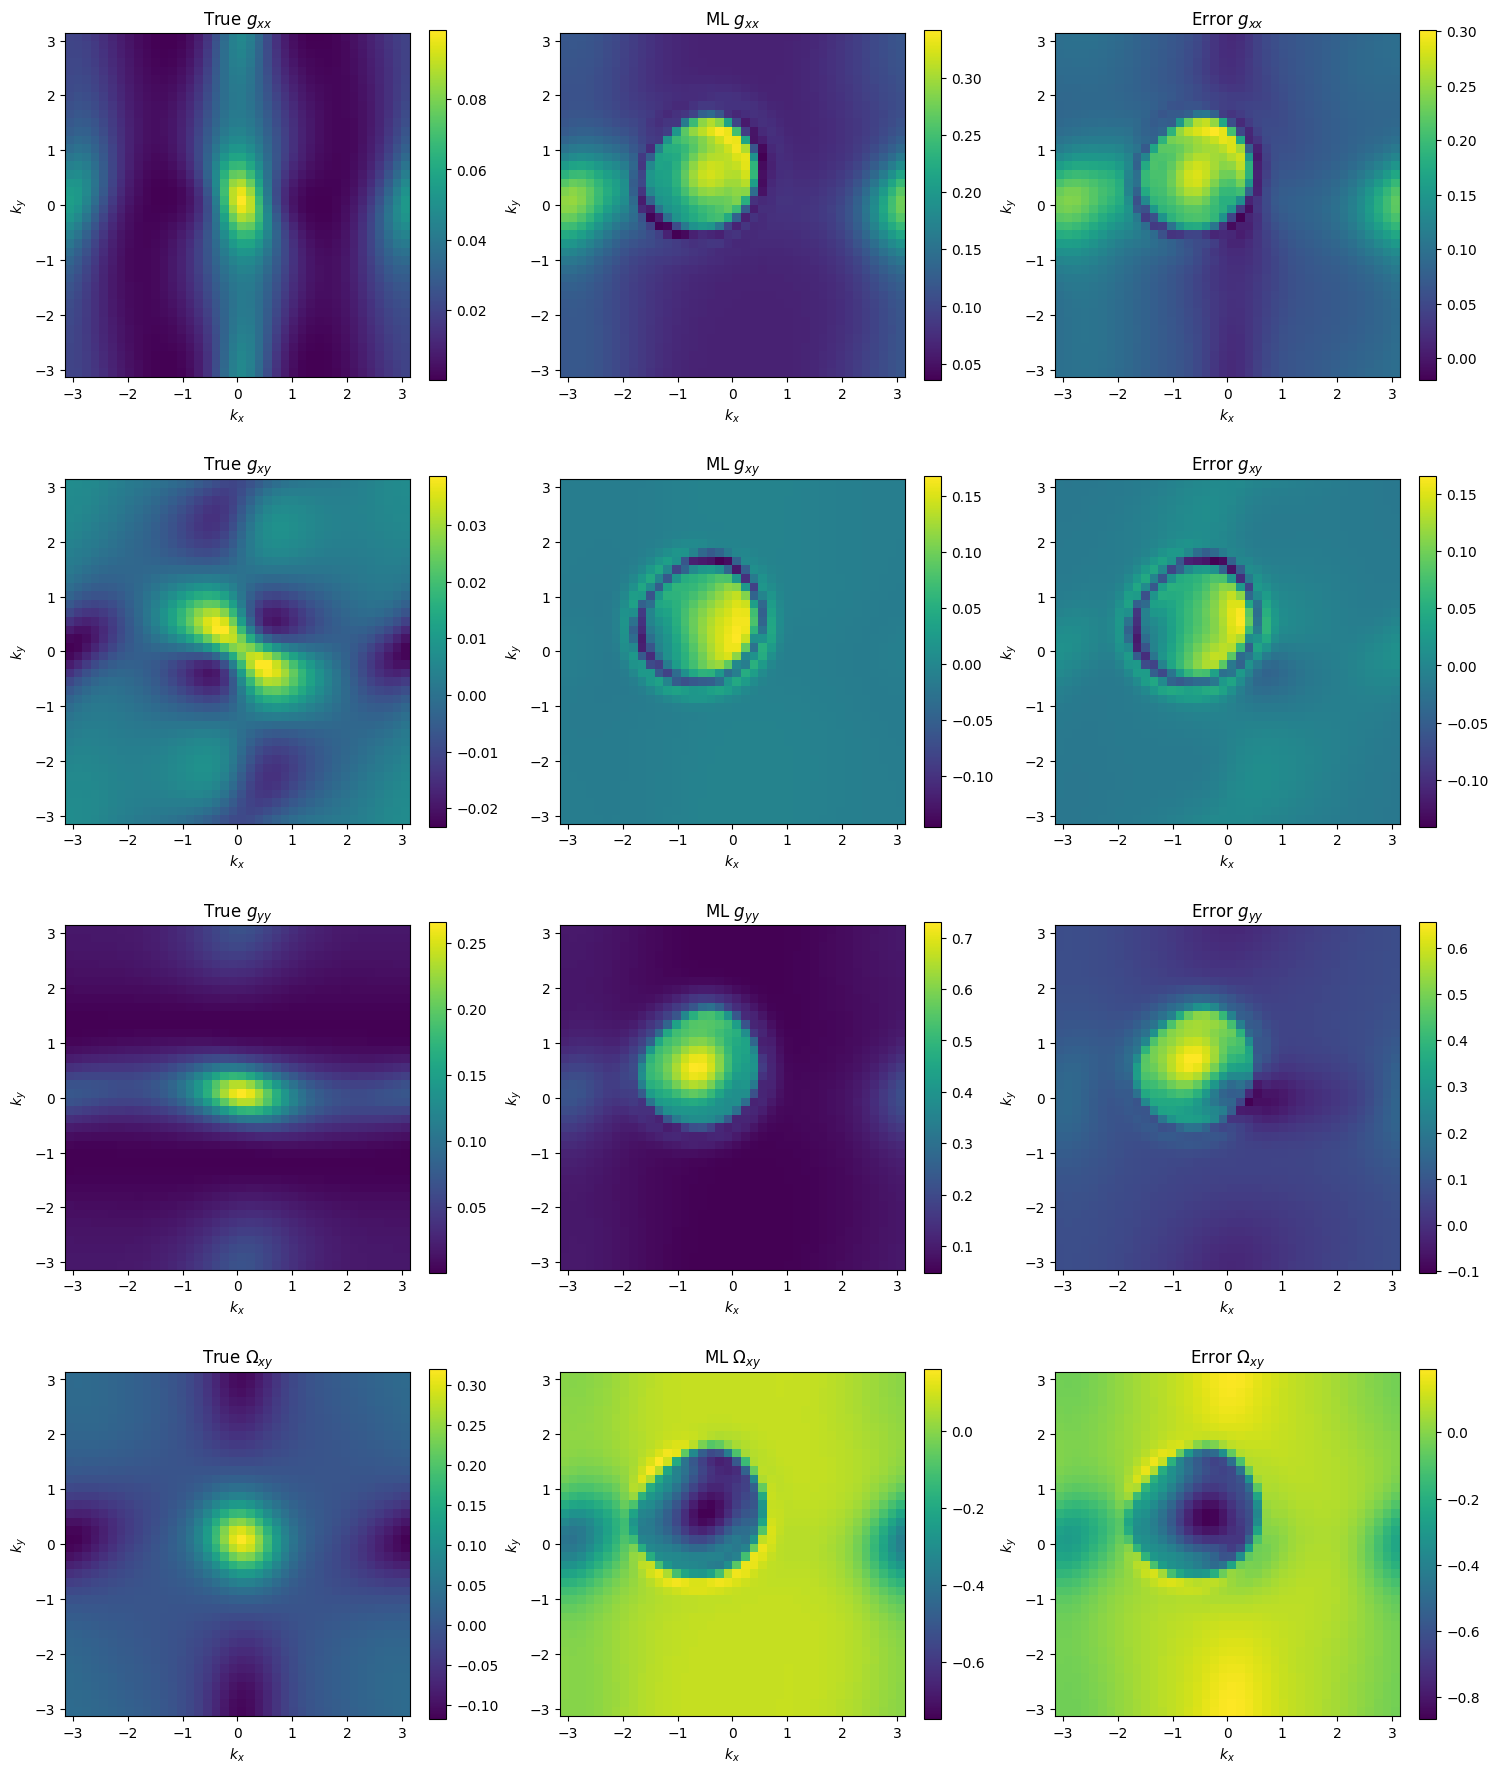
\includegraphics[width=0.47\linewidth,height=2.0cm,keepaspectratio]{QWZ_R1.png}
\hfill
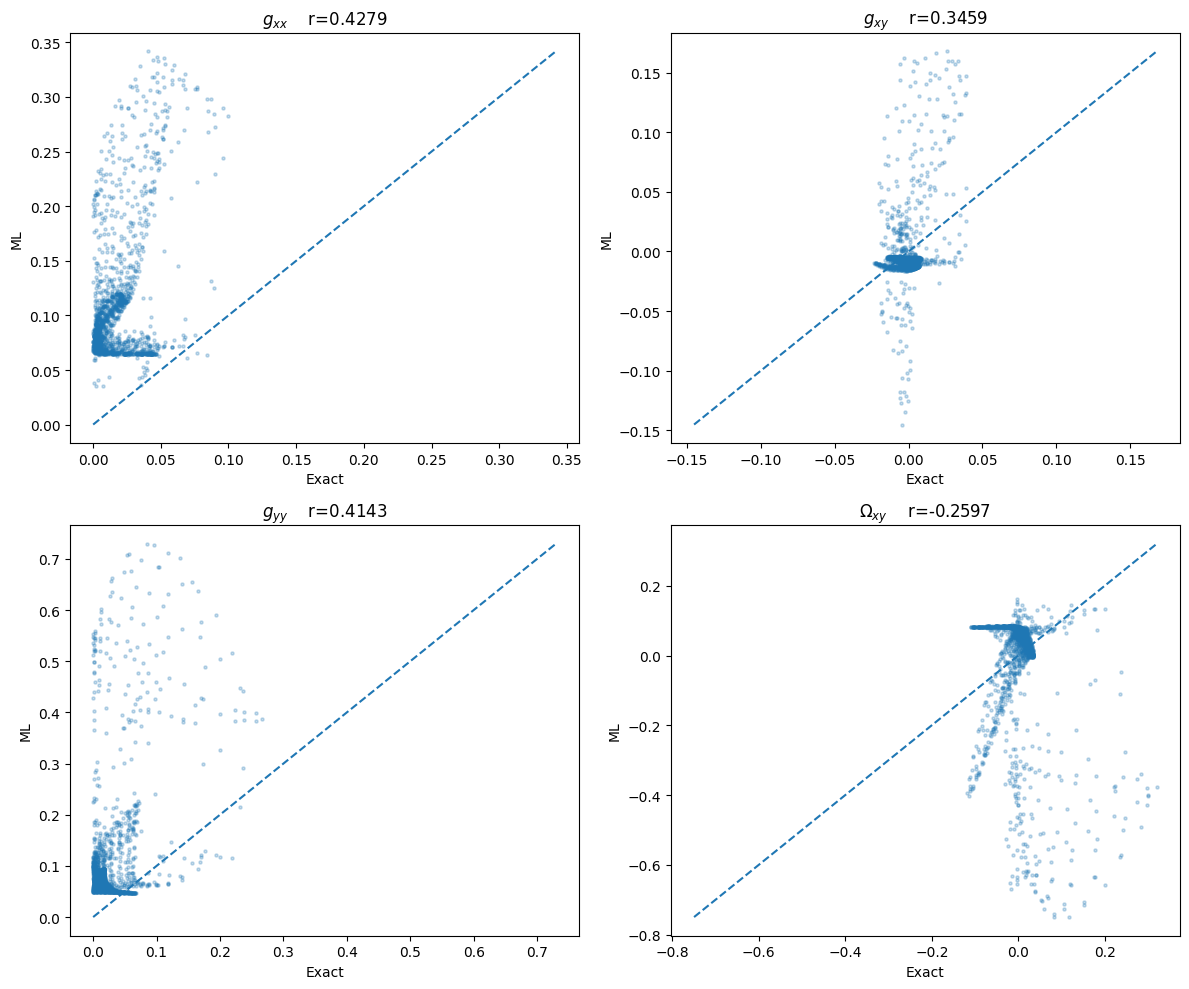
\includegraphics[width=0.47\linewidth,height=2.0cm,keepaspectratio]{QWZ_R2.png}

\vspace{0.08cm}
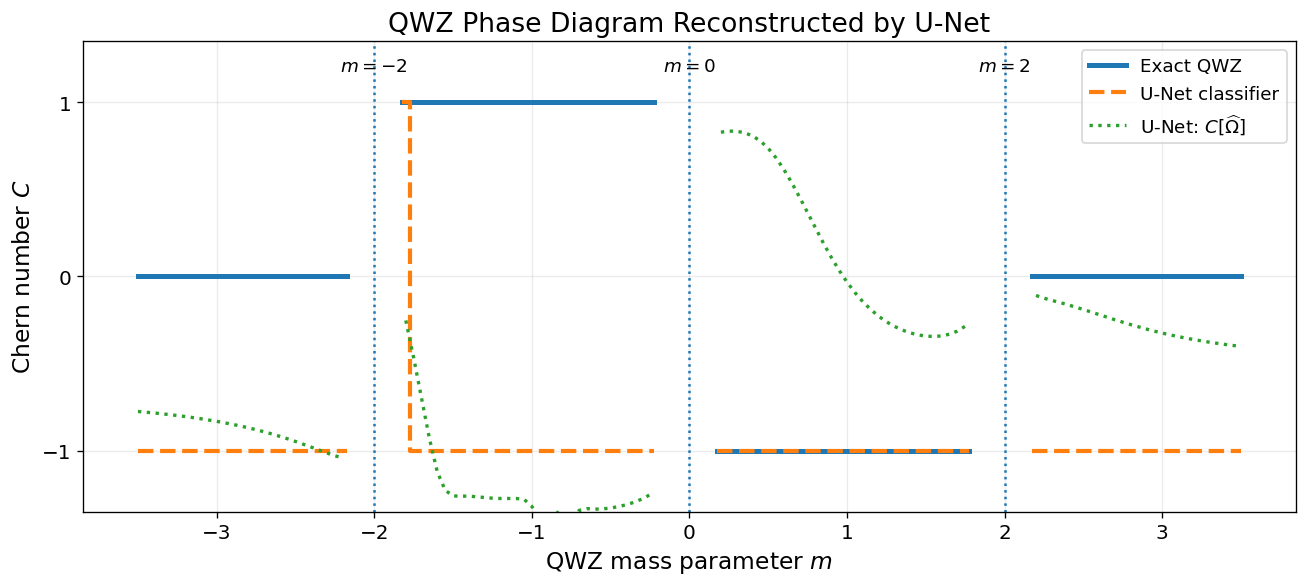
\includegraphics[width=0.78\linewidth,height=2.7cm,keepaspectratio]{QWZ Phase Diagram.png}

{\scriptsize Reconstructed $\Omega^{\ML}_{xy}$, goodness-of-fit, QWZ phase diagram.}
\end{column}
\end{columns}
\end{frame}


% ============================================================
% 5. UNSEEN HAMILTONIAN AND KANE-MELE
% ============================================================
\begin{frame}{5. Generalization: unseen Hamiltonian and Kane--Mele}
\footnotesize

\begin{columns}[T]
\begin{column}{0.56\textwidth}
\textbf{Unseen $C=0$ Hamiltonian} (min gap $2.452$)

\vspace{0.04cm}
\scriptsize
\renewcommand{\arraystretch}{1.08}
\begin{tabular}{@{}lccc@{}}
\toprule
Field & MSE & MAE & MAE/std\\
\midrule
$g_{xx}$ & $1.78\!\times\!10^{-2}$ & 0.111 & 6.63\\
$g_{xy}$ & $2.00\!\times\!10^{-3}$ & 0.0216 & 2.44\\
$g_{yy}$ & $1.70\!\times\!10^{-2}$ & 0.0869 & 2.41\\
$\mathrm{Im}\,Q_{xy}$ & $4.39\!\times\!10^{-2}$ & 0.114 & 4.39\\
$\Omega_{xy}$ & $1.75\!\times\!10^{-1}$ & 0.229 & 4.39\\
\bottomrule
\end{tabular}

\vspace{0.08cm}
\footnotesize
Chern: exact $4.7\!\times\!10^{-10}$; $C^{\ML}_{\rm int}=-0.325$; classifier $=0$ (correct).

Identity $\det g-\Omega^2/4$: true max $3.7\!\times\!10^{-9}$, predicted mean $0.035$.
\end{column}

\begin{column}{0.41\textwidth}
\centering
\textbf{Kane--Mele ($\mathbb Z_2$)}

\vspace{0.04cm}
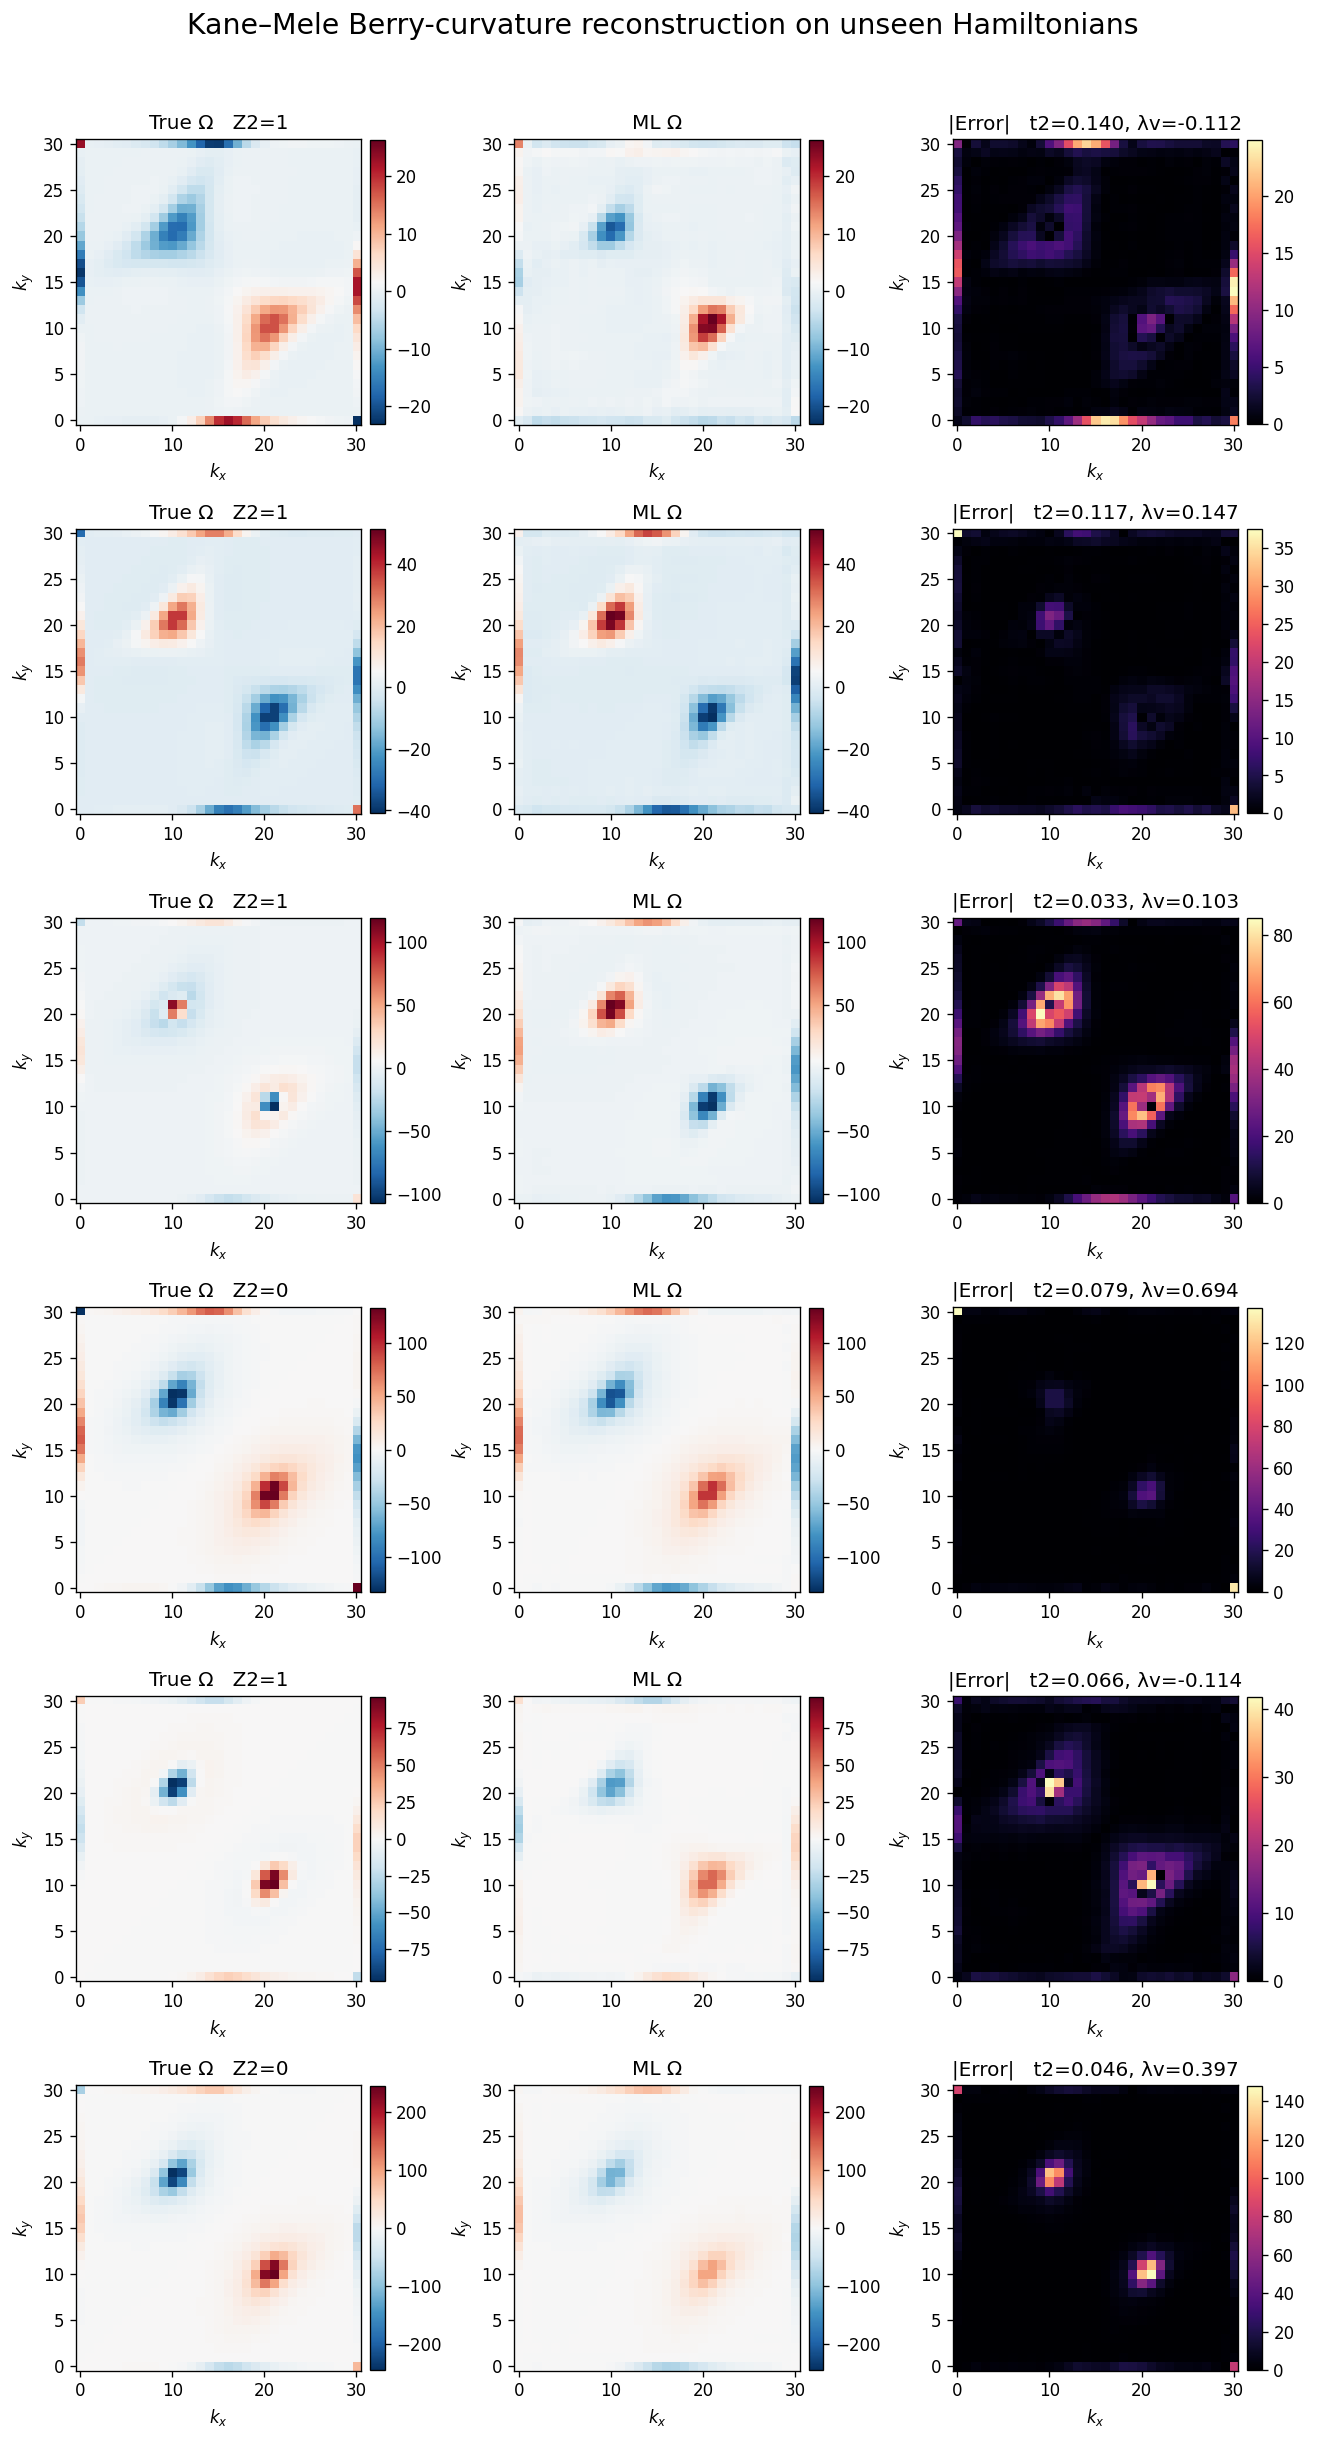
\includegraphics[width=0.48\linewidth,height=2.9cm,keepaspectratio]{Kane Mele Reconstruction.png}
\hfill
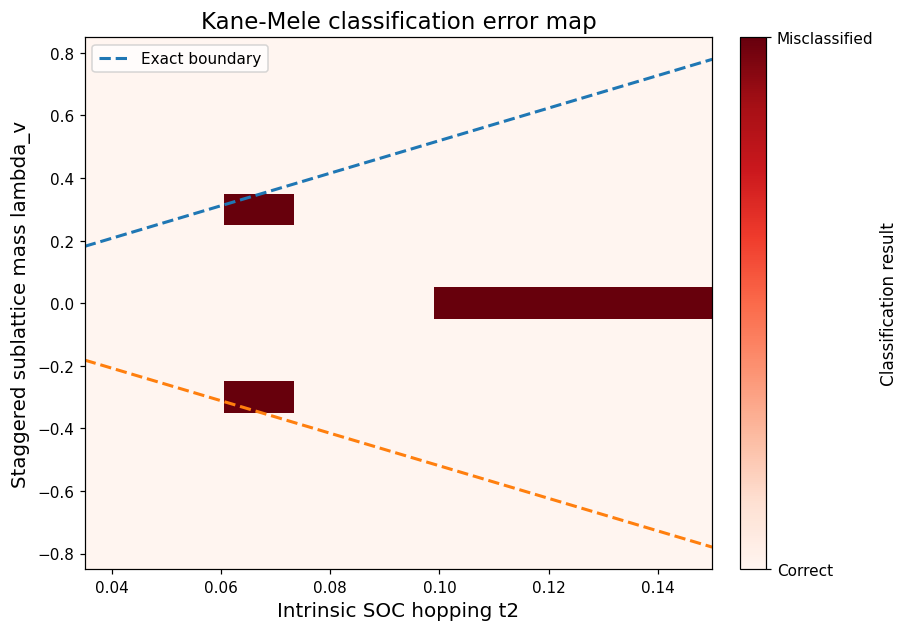
\includegraphics[width=0.48\linewidth,height=2.9cm,keepaspectratio]{Kane Mele Classification Map.png}

\vspace{0.02cm}
{\scriptsize Reconstruction and classification map. Result: $C^{\ML}\simeq-0.153$, $\mathbb Z_2^{\ML}=0$.}
\end{column}
\end{columns}

\vspace{0.08cm}
\begin{ResultBox}\scriptsize\centering
The class label is correct, but MAE/std $>2$ on every field and a $0.035$ identity
residual show the local geometry is not reconstructed faithfully.
\end{ResultBox}
\end{frame}


% ============================================================
% 6. DIAGNOSIS AND TIMELINE
% ============================================================
\begin{frame}{6. Diagnosis and updated timeline}
\footnotesize

\begin{columns}[T]
\begin{column}{0.54\textwidth}
\textbf{Diagnosis from output of the Model: }
\begin{enumerate}
    \item \textbf{Validation is not functioning:} $\mathrm{val}=0.00000$ for all
    100 epochs; final-validation metrics (acc.\ 0.449, $C$-int MAE 0.555,
    round-acc.\ 0.667) equal the epoch-1 train metrics to all printed digits.
    \item Train metrics converge ($C$-cls $=1.000$, $\mathcal L_{\rm topo}=4\!\times\!10^{-5}$),
    but this is not evidence of generalization.
\end{enumerate}
\end{column}

\begin{column}{0.43\textwidth}
\textbf{Completed (Oct 4)}
\begin{itemize}
    \item QWZ data/model and Kane Mele Pipeline.
\end{itemize}

\textbf{Next (by Oct 27)}
\begin{itemize}
    \item Fix validation split/loss; select best checkpoint on held-out data.
    \item Retrain; rerun QWZ scan and unseen tests; regenerate all figures.
    \item Error vs.\ band gap; behaviour near phase boundaries.
    \item More Wannier Hamiltonians $\rightarrow$ multiband.
\end{itemize}
\end{column}
\end{columns}

\vspace{0.08cm}
\begin{ResultBox}\scriptsize\centering
$\mathrm{QWZ}\rightarrow\mathrm{Kane\text{--}Mele}\rightarrow\mathrm{DFT/Wannier}\rightarrow\mathrm{multiband}$;
\textbf{Presentation 3:} transferability + phase-boundary behaviour + interpretation.
\end{ResultBox}
\end{frame}


% ============================================================
% APPENDIX
% ============================================================
\appendix

% ---------- A: QGT ----------
\begin{frame}{Appendix A: Quantum geometric tensor}
\scriptsize
\begin{columns}[T]
\begin{column}{0.47\textwidth}
\[
P(\mathbf k)=\sum_{n\in\mathrm{occ}}|u_n\rangle\langle u_n|,
\qquad
Q_{ij}=\operatorname{Tr}[P(\partial_iP)(\partial_jP)]
\]
\[
Q_{ij}=g_{ij}-\tfrac i2\Omega_{ij},\quad
g_{ij}=\operatorname{Re}Q_{ij},\quad
\Omega_{ij}=-2\operatorname{Im}Q_{ij}
\]
\end{column}
\begin{column}{0.47\textwidth}
Two-band lower band:
\[
g_{ij}=\tfrac14\,\partial_i\hat{\mathbf d}\!\cdot\!\partial_j\hat{\mathbf d},\quad
\Omega_{xy}=-\tfrac12\,\hat{\mathbf d}\!\cdot\!(\partial_x\hat{\mathbf d}\times\partial_y\hat{\mathbf d})
\]
\end{column}
\end{columns}

\vspace{0.1cm}
\textbf{Identity.} $\det g=\tfrac1{16}|\partial_x\hat{\mathbf d}\times\partial_y\hat{\mathbf d}|^2$.
Since $\partial_i\hat{\mathbf d}\perp\hat{\mathbf d}$, the cross product is parallel to $\hat{\mathbf d}$,
so $|\partial_x\hat{\mathbf d}\times\partial_y\hat{\mathbf d}|=|2\Omega_{xy}|$:
\[
\boxed{g_{xx}g_{yy}-g_{xy}^2=\Omega_{xy}^2/4}
\]
Sign of $\Omega_{xy}$ flips between bands. Exact for two-band pure states only.
\end{frame}

% ---------- B: QWZ ----------
\begin{frame}{Appendix B: QWZ model and phase boundaries}
\scriptsize
\begin{columns}[T]
\begin{column}{0.56\textwidth}
\[
d_x=\sin k_x,\quad d_y=\sin k_y,\quad d_z=m+\cos k_x+\cos k_y
\]
\[
E_\pm=\pm\sqrt{\sin^2k_x+\sin^2k_y+(m+\cos k_x+\cos k_y)^2}
\]
Band touching requires $d_x=d_y=d_z=0$, hence $k_x,k_y\in\{0,\pi\}$.
\[
\begin{array}{c|cccc}
\mathbf k&(0,0)&(\pi,0)&(0,\pi)&(\pi,\pi)\\ \hline
d_z&m+2&m&m&m-2
\end{array}
\]
\end{column}
\begin{column}{0.39\textwidth}
\[
\boxed{m=-2,\;0,\;+2}
\]
\[
\boxed{
C^{\ANA}=\begin{cases}
0,&m<-2\\+1,&-2<m<0\\-1,&0<m<2\\0,&m>2
\end{cases}}
\]
\end{column}
\end{columns}
\vfill
\begin{ResultBox}\centering
ML phase boundaries should coincide with $m=-2,0,+2$.
\end{ResultBox}
\end{frame}

% ---------- C: Kane-Mele ----------
\begin{frame}{Appendix C: Kane--Mele phase boundaries}
\scriptsize
\begin{columns}[T]
\begin{column}{0.52\textwidth}
Valley $\eta=\pm1$, spin $s=\pm1$:
\[
H_{\eta s}=v_F(\eta k_x\sigma_x+k_y\sigma_y)+m_{\eta s}\sigma_z
\]
\[
\boxed{m_{\eta s}=\lambda_v-\eta s\,3\sqrt3\,\lambda_{\rm SO}}
\]
\[
E_{\eta s,\pm}=\pm\sqrt{v_F^2k^2+m_{\eta s}^2}
\]
Transition: $m_{\eta s}=0$.
\end{column}
\begin{column}{0.43\textwidth}
\[
\boxed{|\lambda_v|=3\sqrt3\,|\lambda_{\rm SO}|}
\]
\[
\boxed{
\mathbb Z_2^{\ANA}=\begin{cases}
1,&|\lambda_v|<3\sqrt3|\lambda_{\rm SO}|\\
0,&|\lambda_v|>3\sqrt3|\lambda_{\rm SO}|
\end{cases}}
\]
\end{column}
\end{columns}
\vfill
\centering\textbf{Gap closes and reopens at $K/K'$.}
\end{frame}

% ---------- D: BHZ ----------
\begin{frame}{Appendix D: BHZ model and topological criterion}
\scriptsize
\begin{columns}[T]
\begin{column}{0.52\textwidth}
Basis $\{|E1,+\rangle,|H1,+\rangle,|E1,-\rangle,|H1,-\rangle\}$; TRS gives
\[
H_{\rm BHZ}=\begin{pmatrix}h(\mathbf k)&0\\0&h^*(-\mathbf k)\end{pmatrix}
\]
\[
h(\mathbf k)=\epsilon(k)\mathbb 1+Ak_x\sigma_x-Ak_y\sigma_y+M(k)\sigma_z
\]
\[
\epsilon=C-Dk^2,\qquad M=M_0-Bk^2
\]
\end{column}
\begin{column}{0.43\textwidth}
\[
E_\pm=\epsilon\pm\sqrt{A^2k^2+(M_0-Bk^2)^2}
\]
Gap closes at $k=0$ when $\boxed{M_0=0}$.

Mass sign reversal $\mathrm{sgn}\,M(0)\neq\mathrm{sgn}\,M(\infty)$:
\[
\frac{M_0}{B}>0\Rightarrow\text{topological},\quad
\frac{M_0}{B}<0\Rightarrow\text{trivial}
\]
\end{column}
\end{columns}
\vfill
\begin{ResultBox}\centering
$C_\uparrow=-C_\downarrow$, $C_{\rm total}=0$, while $\mathbb Z_2$ can be non-trivial.
\end{ResultBox}
\end{frame}

% ---------- E: boundaries summary ----------
\begin{frame}{Appendix E: Phase boundaries at a glance}
\scriptsize
\begin{columns}[T]
\begin{column}{0.31\textwidth}
\begin{block}{QWZ}
\[\boxed{m=-2,0,+2}\]
\[
C^{\ANA}=\begin{cases}0&m<-2\\+1&-2<m<0\\-1&0<m<2\\0&m>2\end{cases}
\]
\end{block}
\end{column}
\begin{column}{0.36\textwidth}
\begin{block}{Kane--Mele}
\[\boxed{|\lambda_v|=3\sqrt3|\lambda_{\rm SO}|}\]
\[
\mathbb Z_2^{\ANA}=\begin{cases}1&|\lambda_v|<3\sqrt3|\lambda_{\rm SO}|\\0&\text{otherwise}\end{cases}
\]
\end{block}
\end{column}
\begin{column}{0.29\textwidth}
\begin{block}{BHZ}
\[\boxed{M_0=0}\]
\[\tfrac{M_0}{B}>0\Rightarrow\text{topological}\]
\[\tfrac{M_0}{B}<0\Rightarrow\text{trivial}\]
\end{block}
\end{column}
\end{columns}
\end{frame}

% ---------- F: figures ----------
\begin{frame}{Appendix F: Phase-transition figures}
\scriptsize
\begin{columns}[T]
\begin{column}{0.48\textwidth}
\centering
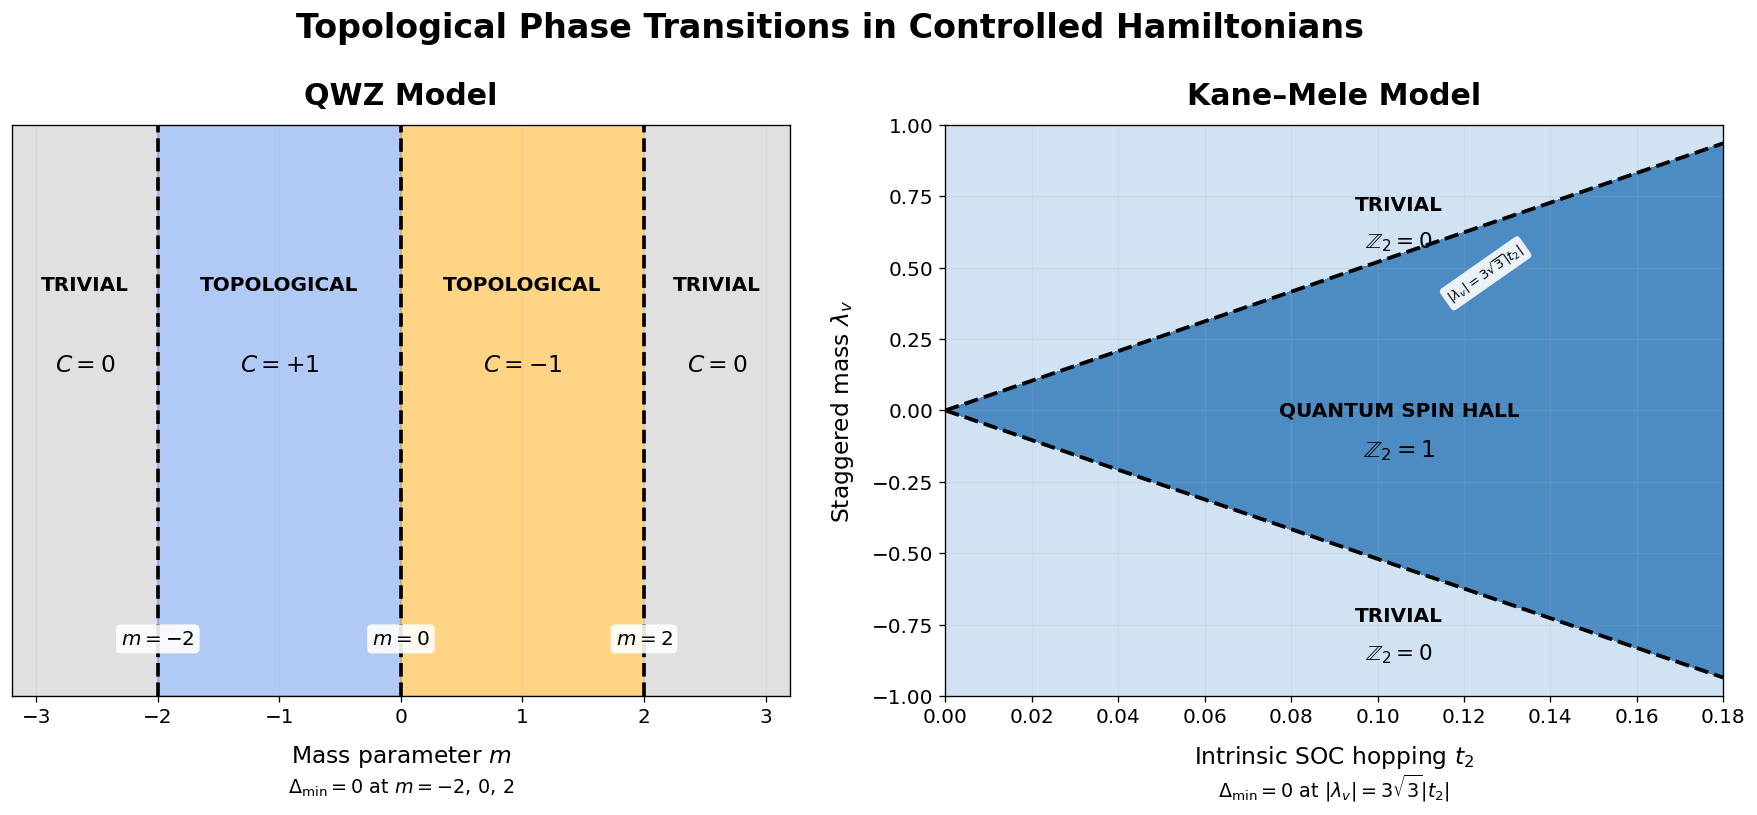
\includegraphics[width=\linewidth,height=2.7cm,keepaspectratio]{Phase Transition Topologica;.png}

QWZ and Kane--Mele transition regimes.

\vspace{0.1cm}
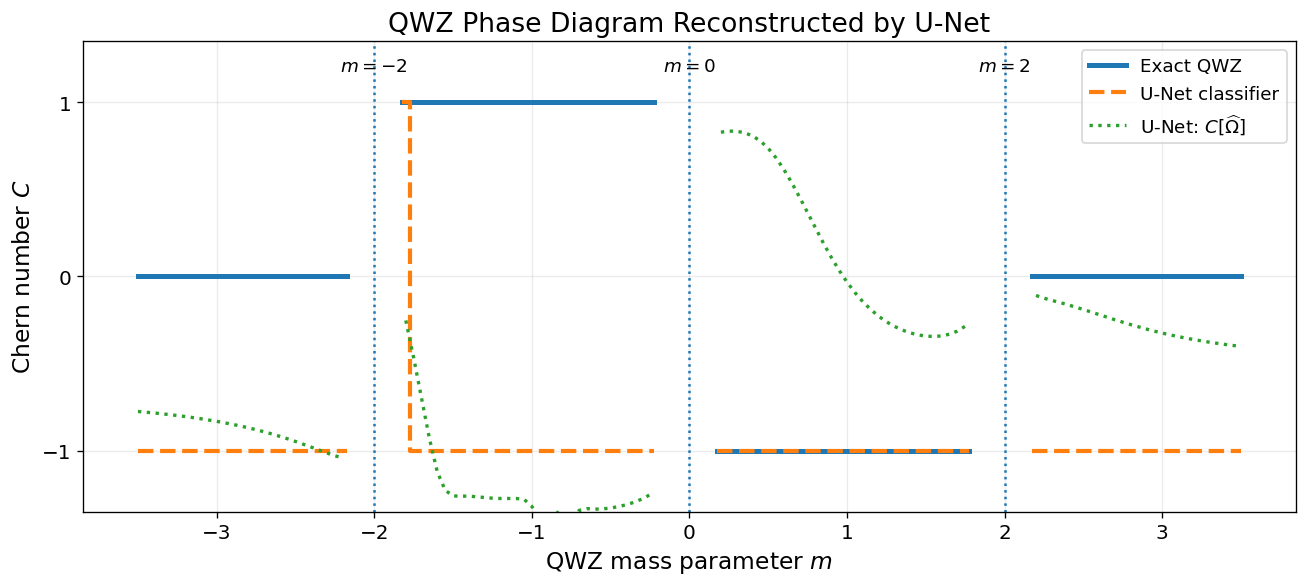
\includegraphics[width=0.85\linewidth,height=2.3cm,keepaspectratio]{QWZ Phase Diagram.png}

QWZ reconstructed ($\ML$) phase diagram.
\end{column}
\begin{column}{0.48\textwidth}
\centering
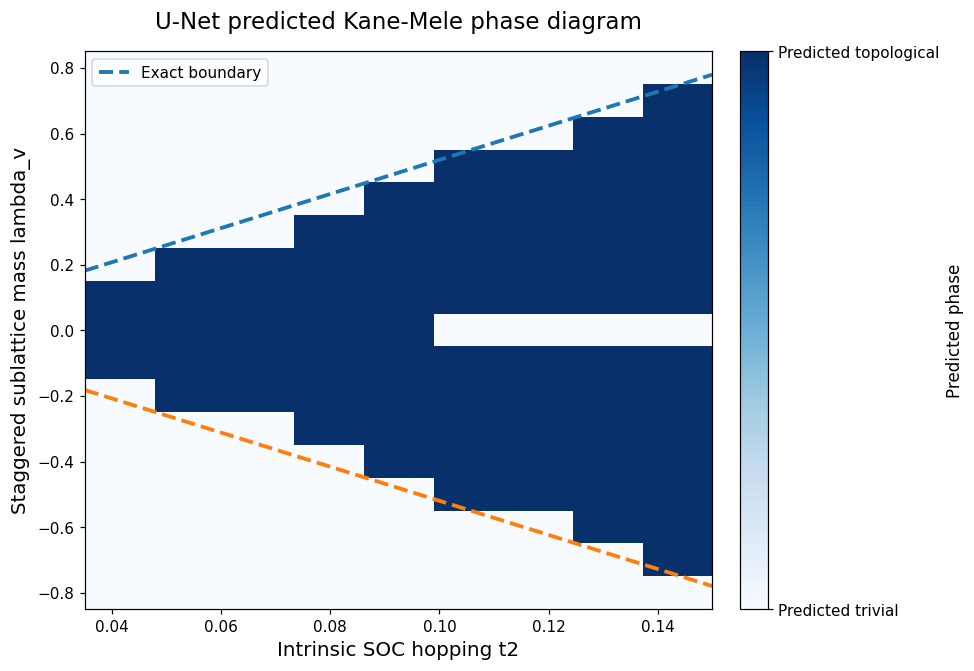
\includegraphics[width=\linewidth,height=2.7cm,keepaspectratio]{U net Phase Diagram kane Mele.png}

Kane--Mele U-Net ($\ML$) phase reconstruction.

\vspace{0.1cm}
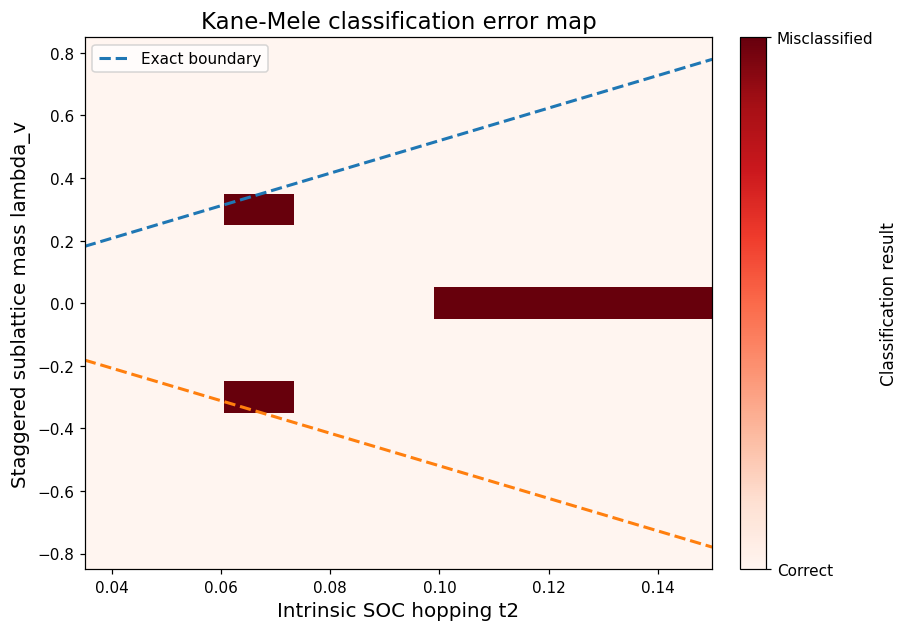
\includegraphics[width=0.85\linewidth,height=2.3cm,keepaspectratio]{Kane Mele Classification Map.png}

Kane--Mele classification ($\mathbb Z_2^{\ML}$).
\end{column}
\end{columns}
\end{frame}

% ---------- G: implementation ----------
\begin{frame}{Appendix G: Implementation summary}
\scriptsize
\textbf{Training family} (14 random coefficients):
\[
\begin{aligned}
d_x&=a_1\sin k_x+a_2\sin k_y+a_3\sin(k_x{+}k_y)+a_4\sin 2k_x,\quad
d_y=b_1\sin k_y+b_2\sin k_x+b_3\sin(k_x{-}k_y)+b_4\sin 2k_y,\\
d_z&=M+\textstyle\sum_{j=1}^{6}c_j\cos(\cdot);\qquad
\text{QWZ: }a_1=b_1=c_1=c_2=1,\ \text{others }0
\end{aligned}
\]
\begin{columns}[T]
\begin{column}{0.50\textwidth}
\textbf{Loss terms}
\[
\mathcal L_{\rm geo}=\big\langle\log\!\big(1+\big|\det g^{\ML}-\tfrac14(\Omega^{\ML}_{xy})^2\big|\big)\big\rangle
\]
\[
\mathcal L_{\rm topo}=\mathrm{SmoothL1}(C^{\ML},C),\quad
C^{\ML}=\tfrac1{2\pi}\textstyle\sum_{\mathbf k}\Omega^{\ML}_{xy}\delta k^2
\]
$\mathcal L_{\rm cls}$: cross-entropy over $C\in\{-1,0,+1\}$.
\end{column}
\begin{column}{0.46\textwidth}
\textbf{Network}
\begin{itemize}
    \item Periodic padding; multi-scale dilated blocks; 3-level U-Net decoder.
    \item High-res.\ local branch fused before QGT head.
    \item Attention pooling $\rightarrow$ Chern head.
\end{itemize}
\textbf{Benchmark:} exact QWZ, 141 values of $m\in[-3.5,3.5]$.
\end{column}
\end{columns}
\end{frame}

% ---------- H: numerics ----------
\begin{frame}{Appendix H: Training milestones and QGT at $\Gamma$}
\scriptsize
\begin{columns}[T]
\begin{column}{0.50\textwidth}
\centering
\textbf{Training milestones (train metrics)}

\vspace{0.05cm}
\begin{tabular}{@{}rccc@{}}
\toprule
Epoch & Total & $\mathcal L_{\rm QGT}$ & C-int MAE\\
\midrule
1 & 6.036 & 0.0291 & 0.555\\
10 & 0.0715 & 0.0102 & 0.0387\\
20 & 0.0723 & 0.0081 & 0.0650\\
50 & 0.0655 & 0.0026 & 0.0853\\
100 & 0.00193 & 0.00030 & 0.0030\\
\bottomrule
\end{tabular}

\vspace{0.05cm}
Validation loss $=0.00000$ in all epochs.
\end{column}

\begin{column}{0.47\textwidth}
\textbf{Full QGT at $\mathbf k=(0,0)$, unseen Hamiltonian}
\[
Q^{\rm true}\!=\!\begin{pmatrix}0.0997&0.0291{-}0.1603i\\0.0291{+}0.1603i&0.2660\end{pmatrix}
\]
\[
Q^{\ML}\!=\!\begin{pmatrix}0.0831&-0.0044{-}0.0600i\\-0.0044{+}0.0600i&0.0550\end{pmatrix}
\]
Off-diagonal imaginary part (curvature) is underestimated by a factor $\approx2.7$.
\end{column}
\end{columns}
\end{frame}

% ---------- I: references ----------
\begin{frame}{Appendix I: References}
\footnotesize
\begin{itemize}
\item \textbf{[Base paper]} A.-K. Wu, L. Primeau, J. Zhang, K. Sun, Y. Zhang and S.-Z. Lin,
``Modeling quantum geometry for fractional Chern insulators with unsupervised learning,''
\textit{npj Comput.\ Mater.} \textbf{12}, 280 (2026), doi:10.1038/s41524-026-02155-1
\item X.-L. Qi, Y.-S. Wu and S.-C. Zhang, \textit{Phys. Rev. B} \textbf{74}, 085308 (2006).
\item C. L. Kane and E. J. Mele, \textit{Phys. Rev. Lett.} \textbf{95}, 146802 (2005).
\item C. L. Kane and E. J. Mele, \textit{Phys. Rev. Lett.} \textbf{95}, 226801 (2005).
\item B. A. Bernevig, T. L. Hughes and S.-C. Zhang, \textit{Science} \textbf{314}, 1757 (2006).
\item NIST JARVIS-DFT database.
\end{itemize}
\end{frame}

\end{document}